\documentclass[12pt]{kiarticle}
\graphicspath{{pictures/}}
\DeclareGraphicsExtensions{.pdf,.png,.jpg,.eps}
%%%
\pagestyle{fancy}
\fancyhf{}
%\renewcommand{\headrulewidth}{ 0.1mm }
\renewcommand{\footrulewidth}{ .0em }
\fancyfoot[C]{\texttt{\textemdash~\thepage~\textemdash}}
\fancyhead[L]{Лабораторная работа № 6.1 \hfil}
\fancyhead[R]{\hfil Иванов Кирилл, 625 группа }
\usepackage{multirow} % Слияние строк в таблице
\newcommand
{\un}[1]
{\ensuremath{\text{#1}}}
\newcommand{\eds}{\ensuremath{ \mathscr{E}}}
\usepackage{tikz}
%%% Работа с таблицами
\usepackage{array,tabularx,tabulary,booktabs} % Дополнительная работа с таблицами
\usepackage{longtable}  % Длинные таблицы
\usepackage{multirow} % Слияние строк в таблице

\begin{document}
	
	\begin{titlepage}
	\begin{center}
		\large 	Московский физико-технический институт \\
		(государственный университет) \\
		Факультет общей и прикладной физики \\
		\vspace{0.2cm}
		
		\vspace{4.5cm}
		Лабораторная работа № 6.1 \\ \vspace{0.2cm}
		\large (Общая физика: квантовая физика) \\ \vspace{0.2cm}
		\LARGE \textbf{Эффект Мессбауэра}
	\end{center}
	\vspace{2.3cm} \large
	
	\begin{center}
		Работу выполнил: \\
		Иванов Кирилл,
		625 группа
		\vspace{10mm}		
		
	\end{center}
	
	\begin{center} \vspace{60mm}
		г. Долгопрудный \\
		2018 год
	\end{center}
\end{titlepage}
	
	\paragraph*{Цель работы:} С помощью метода доплеровского сдвига мессбауэровской линии поглощения исследовать резонансное поглощение $ \gamma $-лучей, испускаемых
	ядрами олова $ ^{119} $ Sn в соединении BaSnO$_3$ при комнатной температуре.
	Определить положение максимума резонансного поглощения, его величина, а также экспериментальная ширина линии $ \Gamma_{экс}$. Оценить время жизни возбуждённого состояния ядра  $^{119}$Sn .
	
	\paragraph*{Оборудование:} 
	
	\section{Теоретическое введение} 
	
	\subsection{Испускание и поглощение в свободных атомах}
	
	\begin{wrapfigure}[20]{l}{0.35\linewidth}
		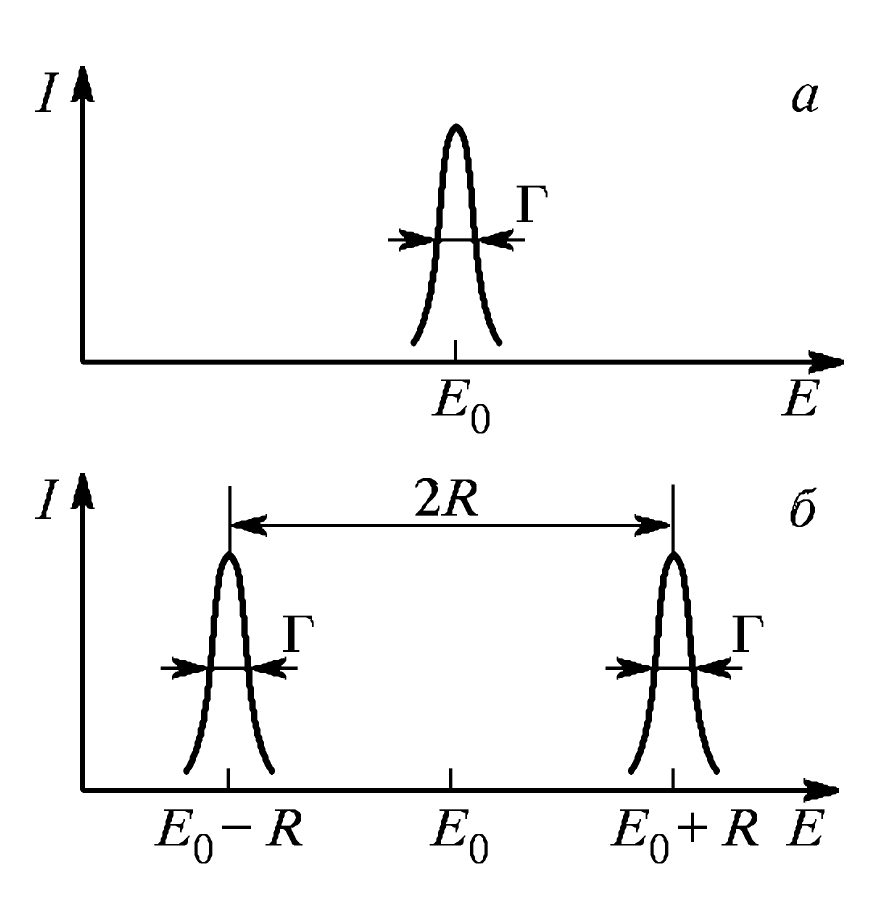
\includegraphics[width=\linewidth]{G}
		\caption{Энергетическое распределение, характеризующее возбужденное состояние ядра (а),
			и сдвиг линий испускания и поглощения из-за отдачи при свободных ядрах (б)}
		\label{ris 1}
	\end{wrapfigure}
	
	Нуклоны (нейтроны и протоны) в атомном ядре, как и электроны
	в атоме, могут находиться в различных дискретных энергетических
	состояниях, или, как говорят, на различных энергетических уровнях.
	Самый низкий из уровней называется основным, остальные носят название возбужденных. Ядра, находящиеся в возбужденных состояниях, могут переходить на более низкие энергетические уровни, в том
	числе и на основной уровень. Такие переходы происходят самопроизвольно (спонтанно). Освобождающаяся энергия уносится фотоном.
	Так возникает $ \gamma $-излучение.
	
	Ядра атомов могут не только испускать, но и поглощать фотоны. Если попадающий в атомное ядро фотон имеет
	энергию, равную разности энергий между основным и каким-либо возбужденным состояниями, то ядро может поглотить фотон и перейти в соответствующее возбужденное состояние. Этот процесс возможен лишь для $ \gamma $-лучей определенных энергий и носит, таким образом, резонансный характер.
	
	На первый взгляд резонансное поглощение  $ \gamma $-лучей должно представлять собой распространенное и легко наблюдаемое явление. Казалось бы, для его обнаружения достаточно пропустить поток $ \gamma $-лучей,
	испущенных радиоактивным источником, через поглотитель, содержащий те же ядра в невозбужденном состоянии. На самом деле это не так. Дело в том, что энергия $E_\gamma $, уносимая $ \gamma $-квантом, оказывается
	меньше энергии $ E_0 $ перехода между уровнями. Небольшая, но вполне
	заметная доля энергии уносится ядром, которое вследствие отдачи начинает двигаться в сторону, противоположную направлению вылета
	$ \gamma $-кванта.
	
	При испускании фотона ядро приобретает энергию отдачи
	
	\begin{equation}\label{R}
	R = \dfrac{p^2}{2M} = \dfrac{E_\gamma^2}{2Mc^2}
	\end{equation}
	
	Для ядра $ ^{119} $Sn, который используется в работе, $E_0 \backsimeq E_\gamma = 23,8 \; кэВ, \; R \backsimeq 2,5 \x 10^{-3} \; эВ \gg \Gamma/2 \backsimeq 3 \x 10^{-8} \; эВ $, где $ \Gamma $ --- естественная ширина линии. Из-за такой разницы в порядках величин получается, что при смещении на величину $ \pm R $ не перекрываются. Однако, это можно компенсировать эффектом Доплера, который возникает из-за теплового движения ядер. Для этого ядра должны двигаться относительно друг друга со скоростью
	
	\begin{equation}\label{V}
	V = c \dfrac{2R}{E_\gamma}
	\end{equation}
	 Это примерно 60 м/с для $ ^{119} $Sn. Из термодинамических соображений оценим скорость движения ядра $ v $:
	
	\begin{equation}\label{}
	\dfrac{Mv^2}{2} = \dfrac{kT}{2} \te v = \sqrt{\dfrac{kT}{M}}
	\end{equation}
	
	Тогда величину $ D $ доплеровского "<уширения"> линии с учетом \eqref{R} можно оценить как
	
	\begin{equation}\label{}
	D = \dfrac{v}{c} E_\gamma = \sqrt{2RkT}
	\end{equation}
	
	При комнатной температуре для $ ^{119} $Sn эта величина будет примерно равна $ 1,5 \x 10^{-2} $ эВ, что на порядок больше $ R $. Происходит перекрытие линий испускания и поглощения вследствие доплеровского уширения. Это обеспечивает возможность резонансного поглощения гамма-лучей.
	
	\subsection{Испускание и поглощение в твердых телах}
	
	Совсем иначе обстоит дело в твердых телах --- в тех веществах с кристаллической решеткой, у которых энергия связи .между атомами в решетке больше энергии отдачи. В таком случае при испускании/поглощении импульс  в том или ином виде передается всем атомам в решетке, что часто вызвает ее колебания. Можно также сказать, что создаются кванты звуковых колебаний --- фононы. 
	
	В данной работе изучается \textbf{эффект Мессбауэра --- испускание и поглощение $ \gamma $-квантов без создания фононов (звуковых колебаний).} Его вероятность выражается формулой 
	
	\begin{equation}\label{}
	f = \exp{-\dfrac{4\pi \langle u^2 \rangle}{\lambda^2}}
	\end{equation}
	
	где $ \langle u^2 \rangle $ --- среднеквадратичное смещение ядер в процессе тепловых колебаний решетки (в направлении вылета $ \gamma $-кванта), $ \lambda $ --- длина волны $ \gamma $-излучения. Таким образом, вероятность упругого испускания (и поглощения) $ \gamma $-квантов уменьшается с температурой (с ростом $  \langle u^2 \rangle $) и с ростом энергии перехода (с уменьшением длины волны $ \lambda $).
	
	Расчеты показывают, что для наблюдения эффекта энергия фотонов должна быть порядка 200 кэВ. Температурный порог может быть разным; в изучаемых нами ядрах олова $ ^{119} $ Sn в соединении BaSnO$_3$ это возможно и при комнатной температуре. Для наблюдения эффекта гамма-излучение сначала пропускается через резонансный поглотитель со стабильными ядрами $ ^{119} $ Sn. Пройдя через него, излучение регистрируется сцинтилляционным спектрометром.  
	
	Наблюдение резонансного поглощения основано на методе доплеровского сдвига линий испускания и поглощения. Для этого поглотителю придается небольшая скорость, рассчитанная по формуле \eqref{V}, где вместо $ R $ подставлена $ \Gamma $. Мессбауэровская линия очень узка, и для наблюдения резонанса хватает скорости порядка миллиметра в секунду. 
	
		\begin{figure}[h!]
		\centering
			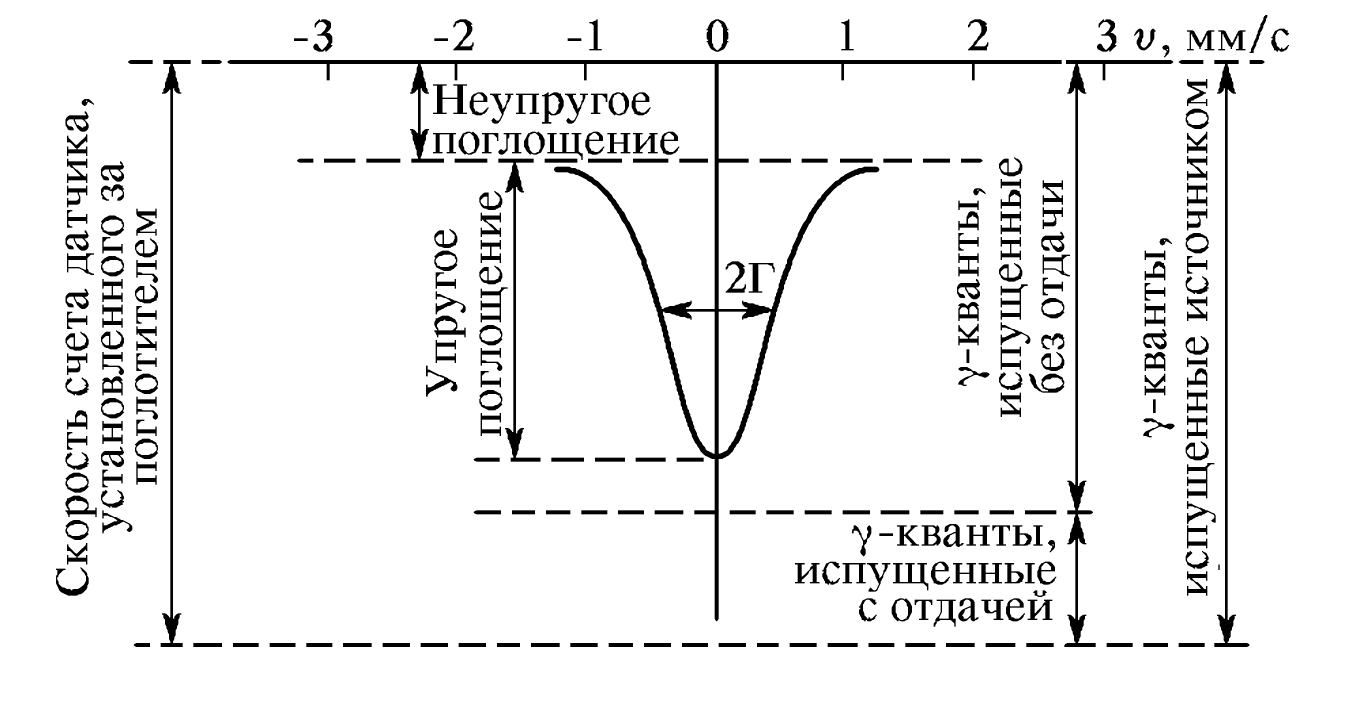
\includegraphics[width=0.7\linewidth]{spektr}
		\caption{Спектр упругого резонансного поглощения $ \gamma $-квантов. Источник и поглотитель находятся в идентичных кристаллических решетках. Неупругое поглощение
			обусловлено главным образом взаимодействием $ \gamma $-лучей с атомными электронами}
		\label{ris 2}
	\end{figure}
	
	Вообще говоря, при идентичных кристаллических решетках, линия испускания полностью перекрывается с линией поглощения, и максимальное поглощение
	наблюдается при нулевой скорости (рис. \ref{ris 2}). Однако в химических сплавах (как наш BaSnO$_3$) из-за влияния электростатических сил происходит смещение максимума поглощения, и его можно "<поймать"> при отличной от нуля скорости. Такое смещение называется \textbf{химическим сдвигом}. Его можно рассчитать по формуле 
	
	\begin{equation}\label{}
	v_p = \dfrac{\Delta E}{E_0}c
	\end{equation}
	
	Для подсчета "<амплитуды"> эффекта Мессбауэра обычно определяется безразмерная величина
	
	\begin{equation}\label{}
	\epsilon(v) = \dfrac{N (\infty) - N(v)}{N (\infty) - N_ф}
	\end{equation}
	
	где $ N(v) $ --- скорость счета квантов, прошедших через поглотитель при
	некоторой скорости $ v $, $ N (\infty) $ --- скорость счета квантов при достаточно
	большой скорости, когда резонансное поглощение отсутствует, $ N_ф  $ --- скорость счета радиоактивного фона.
	
	Измеряемая на опыте ширина резонансной линии $  \Gamma_{экс} $ --- результат наложения линий источника и поглотителя. При тонких поглотителях и источниках и при отсутствии вибраций ширина линии равна удвоенной естественной ширине $ 2\Gamma $ (см. рис. \ref{ris 2}).
	
	\section{Экспериментальная установка}
	
	TODO
	
	\section{Выполнение работы}
	
	TODO
	
	\section{Вывод}
	
	TODO
	
\end{document}